\documentclass[a4paper]{article}

\usepackage[utf8]{inputenc}
\usepackage[T1]{fontenc}
\usepackage{textcomp}
\usepackage{listings}
\usepackage{lmodern}
\usepackage{amsfonts}
\usepackage{titling}
\usepackage{lipsum}
\usepackage[left=1in, right=1in, bottom=1in, top=1in]{geometry}
\usepackage{amsthm}
\usepackage{tcolorbox}
\usepackage{hyperref}
\usepackage{xcolor}
\usepackage{graphicx}
\usepackage{makeidx}
\usepackage{tikz}
\usepackage{cases}
\usepackage{apacite}
\usepackage{tkz-berge}
\usepackage{url}
\usepackage{tgtermes}
\usepackage{sectsty}
\usepackage{subcaption}
\usepackage{setspace}
\usepackage{float}
\usepackage{amsmath, amssymb}


% figure support
\usepackage{import}
\usepackage{xifthen}
\pdfminorversion=7
\usepackage{pdfpages}
\usepackage{transparent}
\usepackage{color}
\newcommand{\incfig}[2][1]{%
    \def\svgwidth{#1\columnwidth}
    \import{./figures/}{#2.pdf_tex}
}

%mathstyling
\theoremstyle{plain}
\newtheorem{thm}{Theorem}[section]
\newtheorem{lem}[thm]{Lemma}
\newtheorem{prop}[thm]{Proposition}
\newtheorem*{cor}{Corollary}

\theoremstyle{definition}
\newtheorem{defn}{Definition}[section]
\newtheorem{conj}{Conjecture}[section]
\newtheorem{exmp}{Example}[section]
\newtheorem{axiom}{Axiom}
\theoremstyle{remark}
\newtheorem*{rem}{Remark}
\newtheorem*{note}{Note}

\definecolor{darkgreen}{rgb}{0.0, 0.5, 0.0}

\pdfsuppresswarningpagegroup=1
\lstset{
tabsize = 4, %% set tab space width
showstringspaces = false, %% prevent space marking in strings, string is defined as the text that is generally printed directly to the console
numbers = left, %% display line numbers on the left
commentstyle = \color{darkgreen}, %% set comment color
keywordstyle = \color{blue}, %% set keyword color
stringstyle = \color{red}, %% set string color
rulecolor = \color{black}, %% set frame color to avoid being affected by text color
basicstyle = \small \ttfamily , %% set listing font and size
breaklines = true, %% enable line breaking
numberstyle = \tiny,
  frame=none,
  xleftmargin=2pt,
  stepnumber=1,
  belowcaptionskip=\bigskipamount,
  captionpos=b,
  escapeinside={*'}{'*},
  language=haskell,
  tabsize=2,
  emphstyle={\bf},
  showspaces=false,
  columns=flexible,
  showstringspaces=false,
  morecomment=[l]\%,
}
\begin{document}
\begin{titlepage}
\begin{center}
\large
University of Warwick \\
Department of Mathematics \\
\huge
\vspace{50mm}
\rule{\linewidth}{0.5pt} \\
MA136 \\
\vspace{5mm}
\Large
Introduction to Abstract Algebra
\rule{\linewidth}{0.5pt}
\vspace{5mm}
\begin{figure}[H]
\centering

\includegraphics[width=0.4\textwidth]{crest_black.eps}
\end{figure}
\vspace{37mm}
Cem Yilmaz \\
\today
\end{center}
\end{titlepage}
\newpage
\tableofcontents
\newpage
\section{Requirements}
\subsection{Functions}
\begin{thm}
	A function is invertible iff it is a bijection
	\begin{proof}
		We know that if $f(x_1) = f(x_2)$, then $x_1=x_2$ in a bijective function, as it is injective. Similarly, from subjectivity, we know that for $y \in Y$ for $f: X \to Y$, there exists  $f(x) = y$. As it is an iff statement, we are required that the proof works in both direction. We first begin with the fact that $f: X \to Y$ is bijective $\implies f$ is invertible. \\
		Suppose that $f$ is invertible, i.e., $\exists g : Y \to X$ such that $f \circ g(y) = y  \; \forall y \in Y$ and $g \circ f (x) = x \; \forall x \in X$. Suppose two elements $x_1,x_2 \in X$ and let us consider $f(x_1)$ and $f(x_2)$. Apply $g$ where
		\begin{align*}
			\implies &g(f(x_1)) = g(f(x_2)) \\
			\implies &g \circ f(x_1) = g\circ f(x_2)\\
			\implies &x_1=x_2 \text{ f is injective}
		\end{align*}
		that is, injectivity follows from the definition of invertible. Now, we show surjectivity. Let $y \in Y$. We know 
		\begin{align*}
			&f \circ g ( y) = y \\
			\implies f(g(y)) =y
		\end{align*}
		Since $g(y) \in X$, $f$ is surjective. In other words, since $g(y)$ is $g : Y \to X$, we show that a unique $x$ mapping does exist. Now, we show that bijectivity implies invertibility also. \\
		Suppose $f$ is a bijective. We need to show that we can construct $g$ such that
		\begin{align*}
			g: Y \to X \\
			f \circ g (y) = y \; \forall y \in Y \\
			g \circ f (x) = x \; \forall x \in X
		\end{align*}
		Let $y \in Y$. Since $f$ is injective and surjective, there exists a unique $x \in X$ such that $f(x) = y$. This gives $g : Y \to  X$. Let $y \in Y$ and consider $f \circ g ( y) = f(g(y))$. By definition of $g$, it follows that
		\begin{align*}
			f(g(y)) = y
		\end{align*}
		Similarly, we consider $x \in X$ and $g\circ f (x) = g(f(x))$. We obtain $g(f(x)) = x$.
	\end{proof}
\end{thm}
\subsection{Matrices}
Let $m,n$ be positive integers. An $m \times n$ matrix (or a matrix of size or order $m \times n$) is a rectangular array consisting of $mn$ numbers arranged in $m$ rows and $n$ columns. The elements are denoted $a_{ij}$ where $i$ is the row and $j$ is the column. The notation for sets of matrices is denoted by $M_{m \times n}(\mathbb{R})$, this is the set of $m \times n$ matrices with entries in $\mathbb{R}$. The addition, subtraction and scalar multiplication is defined in matrices. Whilst addition and subtraction are trivial, the multiplication is to be defined. Let $A = (a_{ij})_{m\times n}$ and $B = (b_{ij})_{n \times p}$, we define the product $AB$ to be the matrix $C = (c_{ij})_{m \times p}$ such that
\begin{align*}
	c_{ij} = a_{i1}b_{i1} + a_{i2}b_{2i} + \ldots + a_{in}b_{nj}
\end{align*}
In other words, multiply the first matrix's row element by corresponding column element. Similarly, we can transform matrices through a function such that 
\begin{align*}
	T_A \begin{bmatrix} x \\ y \end{bmatrix} = A \begin{bmatrix} x \\ y \end{bmatrix}  = \begin{bmatrix} a_{11} & a_{12} \\ a_{21} & a_{22} \end{bmatrix} \begin{bmatrix} x \\ y \end{bmatrix} 
\end{align*}
for $T_A : \mathbb{R}^2 \to  \mathbb{R}^2$. That is, it is something that takes in $\mathbb{R}^2$ and gives back in $\mathbb{R}^2$.Note that these transformations can also be bijective, injective and surjective. For example,
\begin{align*}
	T_A \mathbb{R}^2 \to  \mathbb{R}^2 \\
	T_A(x,y) = \begin{bmatrix} 1 & 2 \\ 3 & 6 \end{bmatrix}  \begin{bmatrix} x \\ y \end{bmatrix}  = \begin{bmatrix} x + 2y \\ 3x+6y \end{bmatrix} 
\end{align*}
Note that this is not surjective as for $x=0$ and $y = 0$ we obtain $(0,0)$ and similarly for $(-2,1)$ we also obtain $(0,0)$. It is also not injective as something such as $(1,4)$ would not have a solution for $x,y$ as the solutions of this transformation lie on $y=3x$.\\
\begin{thm}
	A matrix $A_{2\times 2}$  is invertible if and only if $ad-bc \neq 0$. Then, the inverse is  
	\begin{align*}
		A^{-1} = \frac{1}{ad-bc}\begin{bmatrix} d & -b \\ -c & a \end{bmatrix} 
	\end{align*}
	\begin{proof}
		Let us begin from left to right. We assume $A$ is invertible. This implies the existence of a matrix 
		\begin{align*}
			\begin{bmatrix} x & y \\ z & w \end{bmatrix} \\
			\begin{bmatrix} x & y \\ z & w \end{bmatrix}  \begin{bmatrix} a & b \\ c & d \end{bmatrix}  = \begin{bmatrix} 1 & 0 \\ 0 & 1 \end{bmatrix} 
		\end{align*}
		Therefore the matrix
		\begin{align*}
			\begin{bmatrix} ax+cy & bx + dy \\ az + cw & bz + dw \end{bmatrix}  = \begin{bmatrix} 1 & 0 \\ 0 & 1 \end{bmatrix} 
		\end{align*}
		Hence $ax+cy = 1$, $bx + dy = 0$, $az+cw = 0$ and $bz+dw = 1$. Solving these equations we obtain
		\begin{align*}
			adx+cdy = d& \\
			bcx+dcy = 0& \text{ from multiplying second equation by $c$}\\
			x(ad-bc) = d& \text{ by substitution}
		\end{align*}
		Then, we obtain the second equation
		\begin{align*}
			bax+bcy = b& \text{ by multiplying first equation by $b$}\\
			abx + ady = 0& \text{ by multiplying second equation by $a$}\\
			-(ad-bc)y = b & \text{ by substituting both} \\ 
		\end{align*}
		Then we can further obtain the equations
		\begin{align*}
			(ad-bc) w = a \\
			-(ad-bc)z = c
		\end{align*}
		using further algebra. If $ad-bc=0$, then $a=b=c=d=0$. This means that $A$ is the zero matrix and $A = \underline{0}$, which is not invertible. Therefore, $ad-bc \neq 0$. Hence
		\begin{align*}
			x &= \frac{d}{ad-bc} \\
			y&= \frac{-b}{ad-bc} \\
			w &= \frac{a}{ad-bc} \\
			z &= \frac{-c}{ad-bc}\\
			\begin{bmatrix} x & y \\ z & w \end{bmatrix}  &= \frac{1}{ad-bc}\begin{bmatrix} d & -b \\ -c & a \end{bmatrix} 
		\end{align*}
		Now, RHS to LHS, suppose $ad-bc \neq 0$. Then, let 
		\begin{align*}
			A^{-1} = \frac{1}{ad-bc}\begin{bmatrix} d & -b \\ -c & a \end{bmatrix} 
		\end{align*}
		Then,
		 \begin{align*}
			 A^{-1}A  &= \frac{1}{ad-bc}\begin{bmatrix} d & -b \\ -c & a \end{bmatrix} \begin{bmatrix} a & b \\ c & d \end{bmatrix} \\
				  &= \frac{1}{ad-bc}\begin{bmatrix} ad-bc & 0 \\ 0 & ad-bc \end{bmatrix} \\
				  &= \begin{bmatrix} 1 & 0 \\ 0 & 1 \end{bmatrix} 
		\end{align*}
		Similar steps follow for $A A^{-1}$. Therefore, we have the result in both directions.
	\end{proof}
\end{thm}
As an exercise, let $A$ be a $2\times 2$ matrix where
\begin{align*}
	A = \begin{bmatrix} a & b \\ c & d \end{bmatrix} .
\end{align*}
Let 
\begin{align*}
	u = \begin{bmatrix} a \\ c \end{bmatrix} \;\;\;\;\;\;\;\;\;\;\;\;\;\;\;& v = \begin{bmatrix} b \\ d \end{bmatrix} 
\end{align*}
Show that $|det(A)|$ is the area of the parallelogram with adjacent sides $u$ and $v$. \\
Lastly, we can create a composition of transformations. Suppose two matrices $A = \begin{bmatrix} a_{11} & a_{12} \\ a_{21} & a_{22} \end{bmatrix} $ and $B = \begin{bmatrix} b_{11} & b_{12} \\ b_{21} & b_{22} \end{bmatrix} $. This gives rise to two functions $T_A : \mathbb{R}^2 \to  \mathbb{R}^2$ and $T_B : \mathbb{R}^2 \to  \mathbb{R}^2$. Now,
\begin{align*}
	T_B\left( T_A \begin{bmatrix} x \\ y \end{bmatrix}  \right)  = B \left( A \begin{bmatrix} x \\y \end{bmatrix} \right) &= \begin{bmatrix} b_{11} & b_{12} \\ b_{21} & b_{22} \end{bmatrix} \left( \begin{bmatrix} a_{11} & a_{12} \\ a_{21} & a_{22} \end{bmatrix} \begin{bmatrix} x \\y \end{bmatrix}  \right)
\end{align*}
Would be the same as if we start to multiply wherever. In other words, for $(AB)C = A(BC)$ holds true for $A = m\times n$, $B = n \times p$ and $C = p \times q$ matrix. Matrix multiplication is associative.
\section{Elements of Abstract Algebra}
\subsection{Binary operation}

\begin{defn}
	Binary operation - let $S$ be a set. A binary operation on $S$ is a rule by which any two elements of $S$ can be combined to give another element of $S$. We are giving to use the symbol $\star$ for binary operation. Given $s_1,s_2 \in S$ we have a further element $s_1 \star s_2 \in S$.
	\begin{tcolorbox}[colback=black!3!white,colframe=black!60!white,title=\begin{exmp}Example binary operations \label{Example binary operations}\end{exmp}]
	        Let $S = \mathbb{R}$ and $\star = +$. Then, $x+y \in \mathbb{R}$ indeed, which is an example of a binary operation. However, note that $\mathbb{N}, -$ is not a binary operation as $5-7 = -2 $ and $-2 \not\in \mathbb{N}$.
	\end{tcolorbox}
\end{defn}
	We can also denote the set of all polynomials using the notation
	\begin{align*}
		\mathbb{R}[x]\\
		\mathbb{C}[x]\\
		\mathbb{Q}[x]\\
		\mathbb{Z}[x]
	\end{align*}
	These would denote the set of all polynomials whose coefficients follow the set in the notation. Note that addition and subtraction on polynomials is a binary operation. \\
	Note that composition of functions is not a binary operation. For example, $f : A\to B$ and $g: B\to C$ then $g \circ f : A \to C$ is not a binary operation due to difference in set mappings. 
\subsection{Commutativity}
\begin{defn}
	Let $S$ be a set and $\star$ a binary operation. We say that the binary operation $\star$ is commutative on $S$ if
	\begin{align*}
	a \star b = b \star a	
	\end{align*}
	for all $a,b \in S$
\end{defn}
\begin{tcolorbox}[colback=black!3!white,colframe=black!60!white,title=\begin{exmp}Examples of commutativity \label{Examples of commutativity}\end{exmp}]
        For example, $\mathbb{R},+$ is commutative
\end{tcolorbox}
\subsection{Associativity}
\begin{defn}
We say that a binary operation $\star$ is associative on $S$ if
\begin{align*}
	(a \star b) \star c = a \star (b \star c)
\end{align*}
for all $a,b,c \in S$. I.e., bracketing doesn't matter as long as we keep the same order and this is called the general associativity theorem.
\begin{tcolorbox}[colback=black!3!white,colframe=black!60!white,title=\begin{exmp}Examples of associativity \label{Examples of associativity}\end{exmp}]
        For example, $\mathbb{R}, +$ is also associative
\end{tcolorbox}
\end{defn}
\subsection{Groups}
\begin{defn}
	A group is a pair $(G, \star)$ where $G$ is a set and $\star$ is a binary operation on $G$, such that the following four properties hold:
	\begin{enumerate}
		\item closure - $\forall a,b \in G$, $a \star b \in G$.
		\item associativity - $\forall a,b,c \in G$, $a \star ( b \star c )  = (a \star b) \star c$
		\item existence of identity element - $\exists e . \forall  a \in G, a \star e = e \star a = a$ 
		\item existence of inverse - $\forall a \in G, \exists  b \in G . a \star b = b \star a = e$
	\end{enumerate}
\end{defn}
\begin{defn}
	A group is called Abelian if it is a group and follows
	\begin{enumerate}
		\item commutative - $\forall a,b \in G, a \star b = b \star a$
	\end{enumerate}
\end{defn}
\begin{tcolorbox}[colback=black!3!white,colframe=black!60!white,title=\begin{exmp}Example of Groups \label{Example of Groups}\end{exmp}]
        Some example groups are:
	\begin{enumerate}
		\item $(\mathbb{R},+)$ 
	\end{enumerate}
\end{tcolorbox}
We can also form groups of the same binary operation by picking only specific elements. I.e.,
\begin{defn}
	A subgroup is a group with the same binary operation $\star$ but it uses the specific set $X$ where $X \subseteq G$.
\end{defn}
We get something of the kind
\begin{figure}[H]
	\centering
	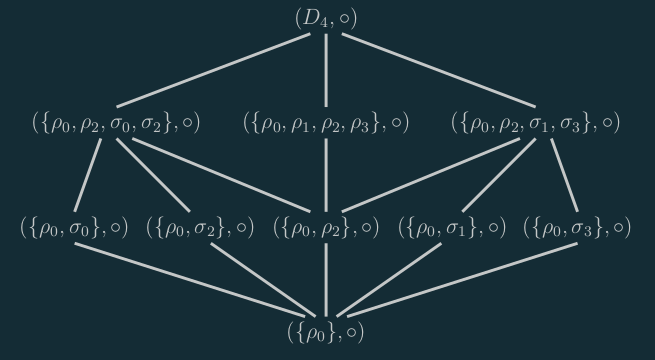
\includegraphics[width=0.8\textwidth]{sub.png}
	\caption{Subgroup}
	\label{fig:sub-png}
\end{figure}
Furthermore,
\begin{thm}
	Uniqueness of the identity element. Let $(G, \star)$ be a group. Then $(G, \star)$ has a unique identity element. 
	\begin{proof}
		Let $a \in G$. Suppose $b,b' \in G$ which are both inverses to $a$. Then,
		\begin{align*}
			b \star a = a \star b = e \\
			b' \star a = a \star b' = e \\
			b = b \star e = b \star (a \star b') \\
			b = (b\star a) \star b' = b = e \star b'\\
			b = b'
		\end{align*}
	\end{proof}
		
\end{thm}
\begin{thm}
	Inverse of an inverse. Let $G$ be a group and $a \in G$. Then
	\begin{align*}
		(a^{-1})^{-1} = a
	\end{align*}
	\begin{proof}
		Let $a \in G$. Need to show $a$ is the inverse of $a^{-1}$. This means that $a^{-1}a = aa^{-1}=e$. Hence
		\begin{align*}
			(a^{-1})^{-1}
		\end{align*}
	\end{proof}
\end{thm}
\begin{thm}
	Inverse of a product. Let $G$ be a group and $a,b \in G$. Then,
	\begin{align*}
		(ab)^{-1} = b^{-1}a^{-1}
	\end{align*}
	\begin{proof}
		$b^{-1}a^{-1}$ is the inverse of $ab$.
		\begin{align*}
			(ab)(b^{-1}a^{-1}) & abb^{-1}a^{-1} \\
					   &=a 1 a^{-1}\\
					   &= aa^{-1} \\
					   &= 1 
		\end{align*}
	\end{proof}
\end{thm}
\begin{thm}
	Properties of power notation. Let $G$ be a group and let $a \in G$. Then
	\begin{enumerate}
		\item $a^{n}\in G$ for all $n \in \mathbb{Z}$.
		\item If $n \in \mathbb{Z}$ then $(a^{-1})^{n} = (a^{n})^{-1}= a^{-n}$ 
		\item Moreover, if $m,n$ are integers then $(a^{m})^{n} = a^{mn}$ and $a^{m}a^{n}=a^{m+n}$ 
		\item Further, if the group $G$ is abelian, $a,b \in G$ and $n $ is an integer then $(ab)^{n}=a^{n}b^{n}$
	\end{enumerate}
	Proof for $1$ 
	\begin{proof}
		$a^{0}=1$, true for $n=0$. Suppose $n>0$, $n \in \mathbb{Z}$. For $n=1$, $a^{n}=a$ and indeed $a \in G$. Assume true if $n=k$, $k>0$, $k \in \mathbb{Z}$. Consider
		\begin{align*}
			a^{k+1} = a^{k}a
		\end{align*}
		Certainly $a^{k}a \in G$ as $a \in G$ and $a^{k} \in G$ by assumption. Suppose $n<0$, $n \in \mathbb{Z}$. We know
		\begin{align*}
			a^{n} = (a^{-n})^{-1}
		\end{align*}
		As $-n > 0$ by earlier, we know $a^{-n}\in G \implies (a^{-n})^{-1} \in G$.
	\end{proof}
	Proof for $2$ 
	\begin{proof}
		If $n=0$, $(a^{-1})^{0}= (a^{0})^{-1}= a^{-0}$ Indeed, all of these are equal to the identity $e$. If $n>0$, $n \in \mathbb{Z}$, we consider $a^{n}(a^{-1})^{n}$:
		\begin{align*}
			a^{n}(a^{-1})^{n} = \underbrace{aa\ldots a}_{n}\underbrace{a^{-1}a^{-1}\ldots a^{-1}}_{n} \\
			a^{n}(a^{-1})^{n}=\underbrace{11\ldots 1}_{n} \\
			a^{-n} = (a^{n})^{-1}
		\end{align*}
		Suppose $n<0$ and $n \in \mathbb{Z}$. Suppose $a^{n}(a^{-1})^{n}$:
		\begin{align*}
			a^{n}(a^{-1})^{n} &= (a^{-n})^{-1}\left( (a^{-1})^{-n} \right) ^{-1} \\
					  &= (a^{-1})^{-n}\left( (a^{-1})^{-1} \right) ^{-n}\\
					  &= (a^{-1})^{-n}a^{-n} \\
					  &= \underbrace{aa\ldots a}_{n}\underbrace{a^{-1}a^{-1}\ldots a^{-1}}_{n} \\
		\end{align*}
	\end{proof}
	Proof for $3$ 
	
\end{thm}
\end{document}
